% Titelseite
\DeclareNewLayer[background,%
  width=115mm,%
  height=158mm,%
  hoffset=5mm,%
  voffset=5mm,%
  contents={%
   \begin{tikzpicture}[x=1mm, y=1mm]%
      % map image
      \draw (0,0) node [inner sep=0mm, anchor=south west] {%
        
\includegraphics[height=158mm]{images-print/Entwurf_Titelbild_A6.pdf}%
      };%
      \end{tikzpicture}%
   }%
]{titelseite}
\newpairofpagestyles[]{page-title}{}
\AddLayersAtBeginOfPageStyle{page-title}{titelseite}
\AddLayersAtBeginOfPageStyle{page-title}{cropmarksplain}

% Campuskarte
\DeclareNewLayer[background,%
  width=115mm,%
  height=158mm,%
  hoffset=5mm,%
  voffset=5mm,%
  contents={%
    \begin{tikzpicture}[x=1mm, y=1mm]%
      % map image
      \draw (0,0) node [inner sep=0mm, anchor=south west] {%
        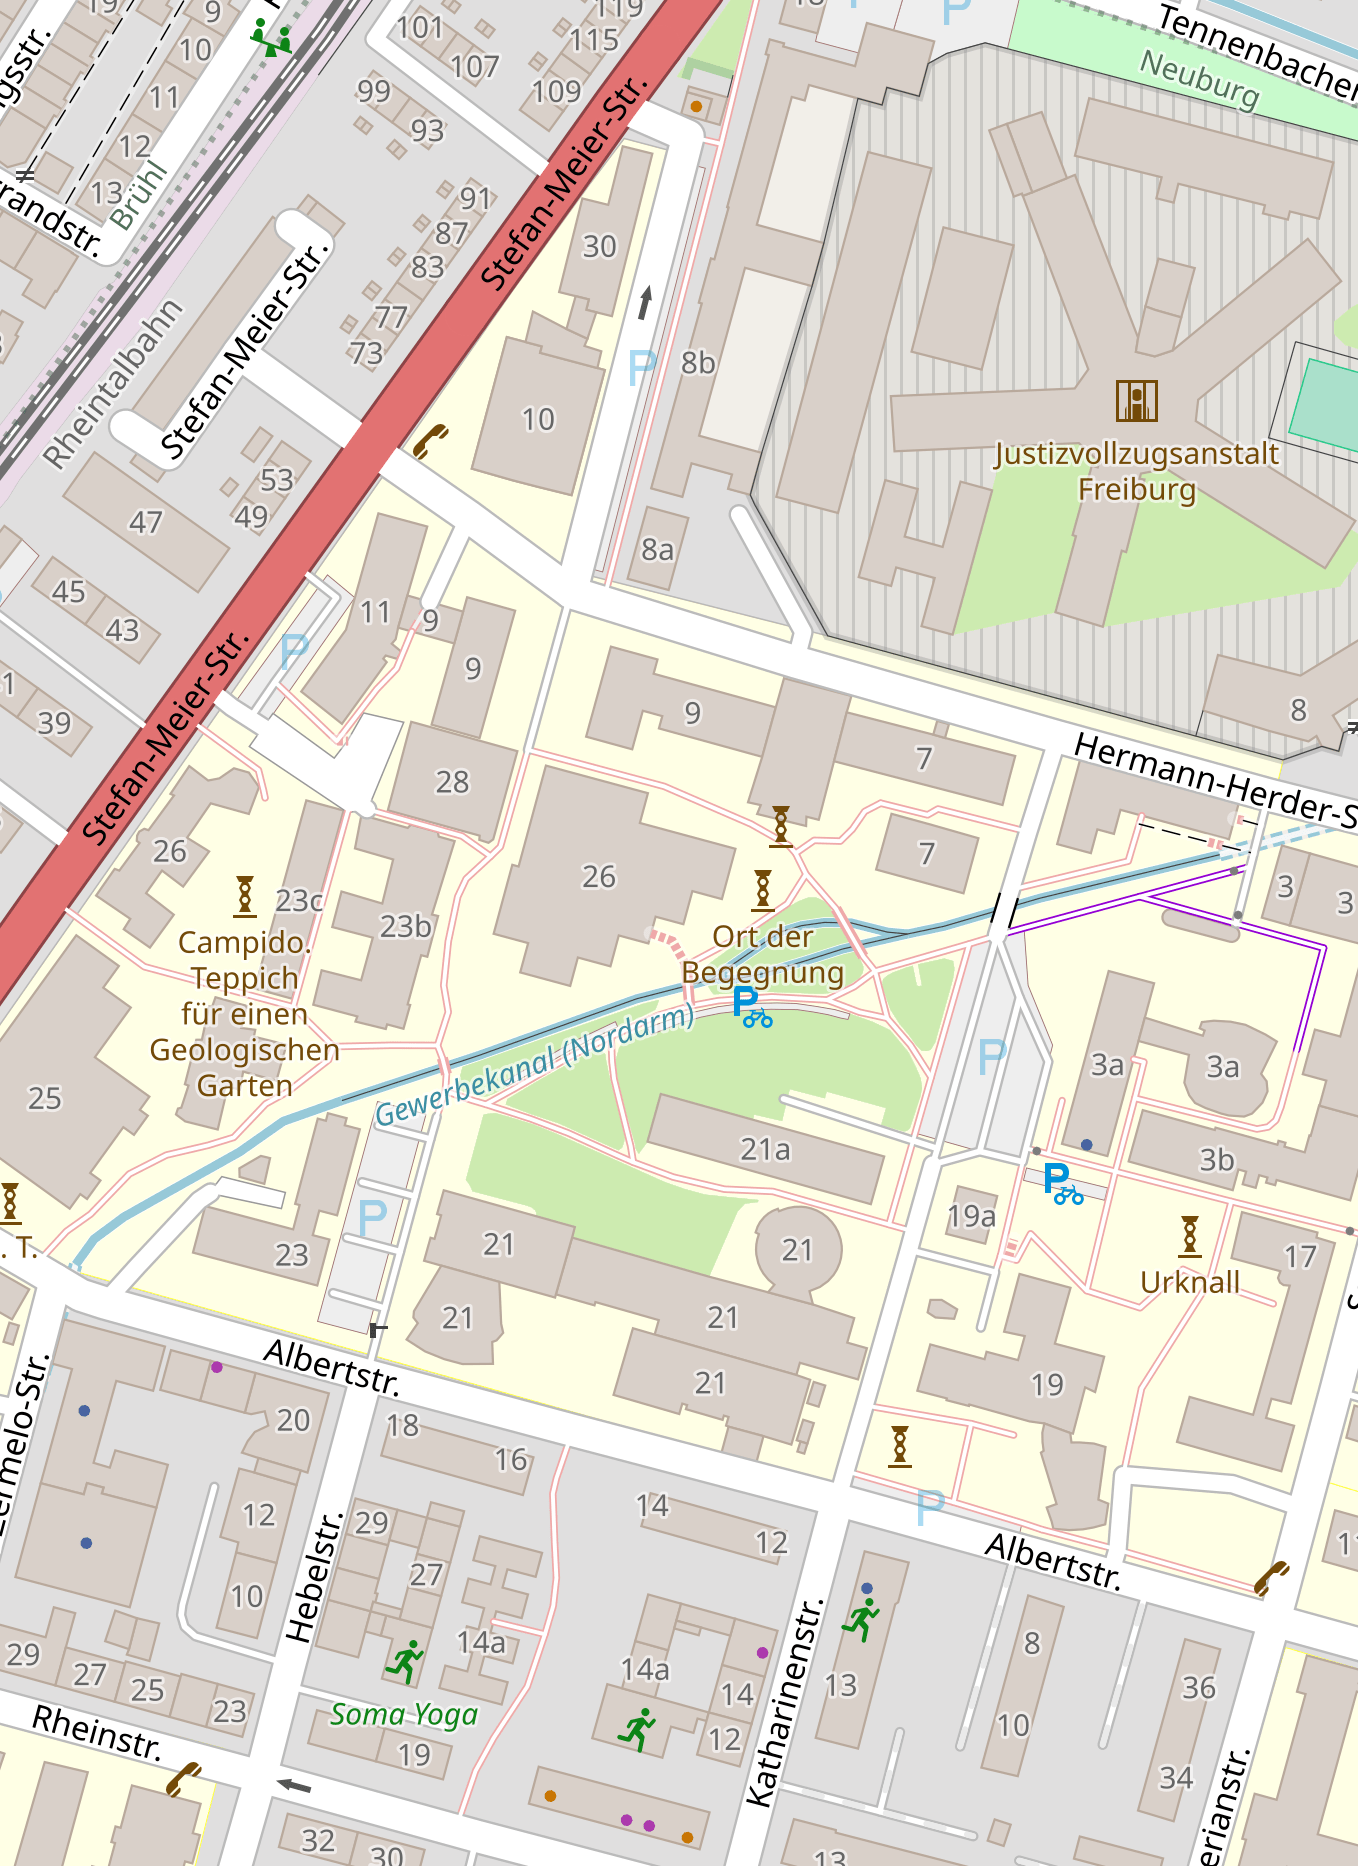
\includegraphics[width=115mm]{images-print/freiburg-campus.png}%
      };%
      % box for map key
      \fill [white] (0,39) rectangle (52,0);%
      % map key text
      \draw (8,8) node [anchor=south west, align=left] {%
        \begin{minipage}{47mm}%
          \small
          1 Hörsaal Rundbau \linebreak
          2 Ausstellung, Welcome Desk \linebreak
          3 Hörsaal Anatomie \linebreak
          4 Hörsaal Weismannhaus \linebreak
          5 Workshopräume \linebreak
          6 Hermann-Herder-Str. 9, R\,00\,020\linebreak
          7 Albertstr. 21, R\,00\,004\linebreak
          8 Mensa
        \end{minipage}%
      };
      % circles with numbers
      \node (1) at (67.00,49.50) [] {}; % HS Rundbau
      \node (1label) at (1) [fill=geoblau, draw=black, inner sep=0.3mm, circle] {1}; % HS Rundbau
      \node (2) at (64.00,40.00) [] {}; % Chemie-Hochhaus
      \node (2label) at (2) [fill=white, draw=black, inner sep=0.3mm, circle] {2}; % Chemie-Hochhaus
      \node (3) at (91.50,33.50) [] {}; % HS Anatomie
      \node (3label) at (3) [fill=hellgelb, draw=black, inner sep=0.3mm, circle] {3}; % HS Anatomie
      \node (4) at (69.50,59.00) [] {}; % HS Weismannhaus
      \node (4label) at (4) [fill=hellgruen, draw=black, inner sep=0.3mm, circle] {4}; % HS Weismannhaus
      \node (5) at (45.00,119.50) [] {}; % Workshopräume
      \node (5label) at (5) [fill=dezentrot, draw=black, inner sep=0.3mm, circle] {5}; % Workshopräume
      \node (6) at (55.00,98.50) [] {}; % BoF 1
      \node (6label) at (6) [fill=white, draw=black, inner sep=0.3mm, circle] {6}; % BoF 2
      \node (7) at (55.00,49.00) [] {}; % BoF 2
      \node (7label) at (7) [fill=white, draw=black, inner sep=0.3mm, circle] {7}; % BoF 2
      \node (8) at (51.00,87.00) [] {}; % Mensa
      \node (8label) at (8) [fill=white, draw=black, inner sep=0.3mm, circle] {8}; % Mensa
    \end{tikzpicture}%
  }%
]{campuskarte}
\newpairofpagestyles[]{page-campuskarte}{}
\AddLayersAtBeginOfPageStyle{page-campuskarte}{campuskarte}
\AddLayersAtBeginOfPageStyle{page-campuskarte}{cropmarksplain}

% Raumplan Erwin-Schrödinger-Zentrum
\DeclareNewLayer[background,%
  width=115mm,%
  height=158mm,%
  hoffset=5mm,%
  voffset=5mm,%
  contents={%
    \begin{tikzpicture}[x=1mm, y=1mm]%
      % map image
      \draw (0,0) node [inner sep=0mm, anchor=south west] {%
        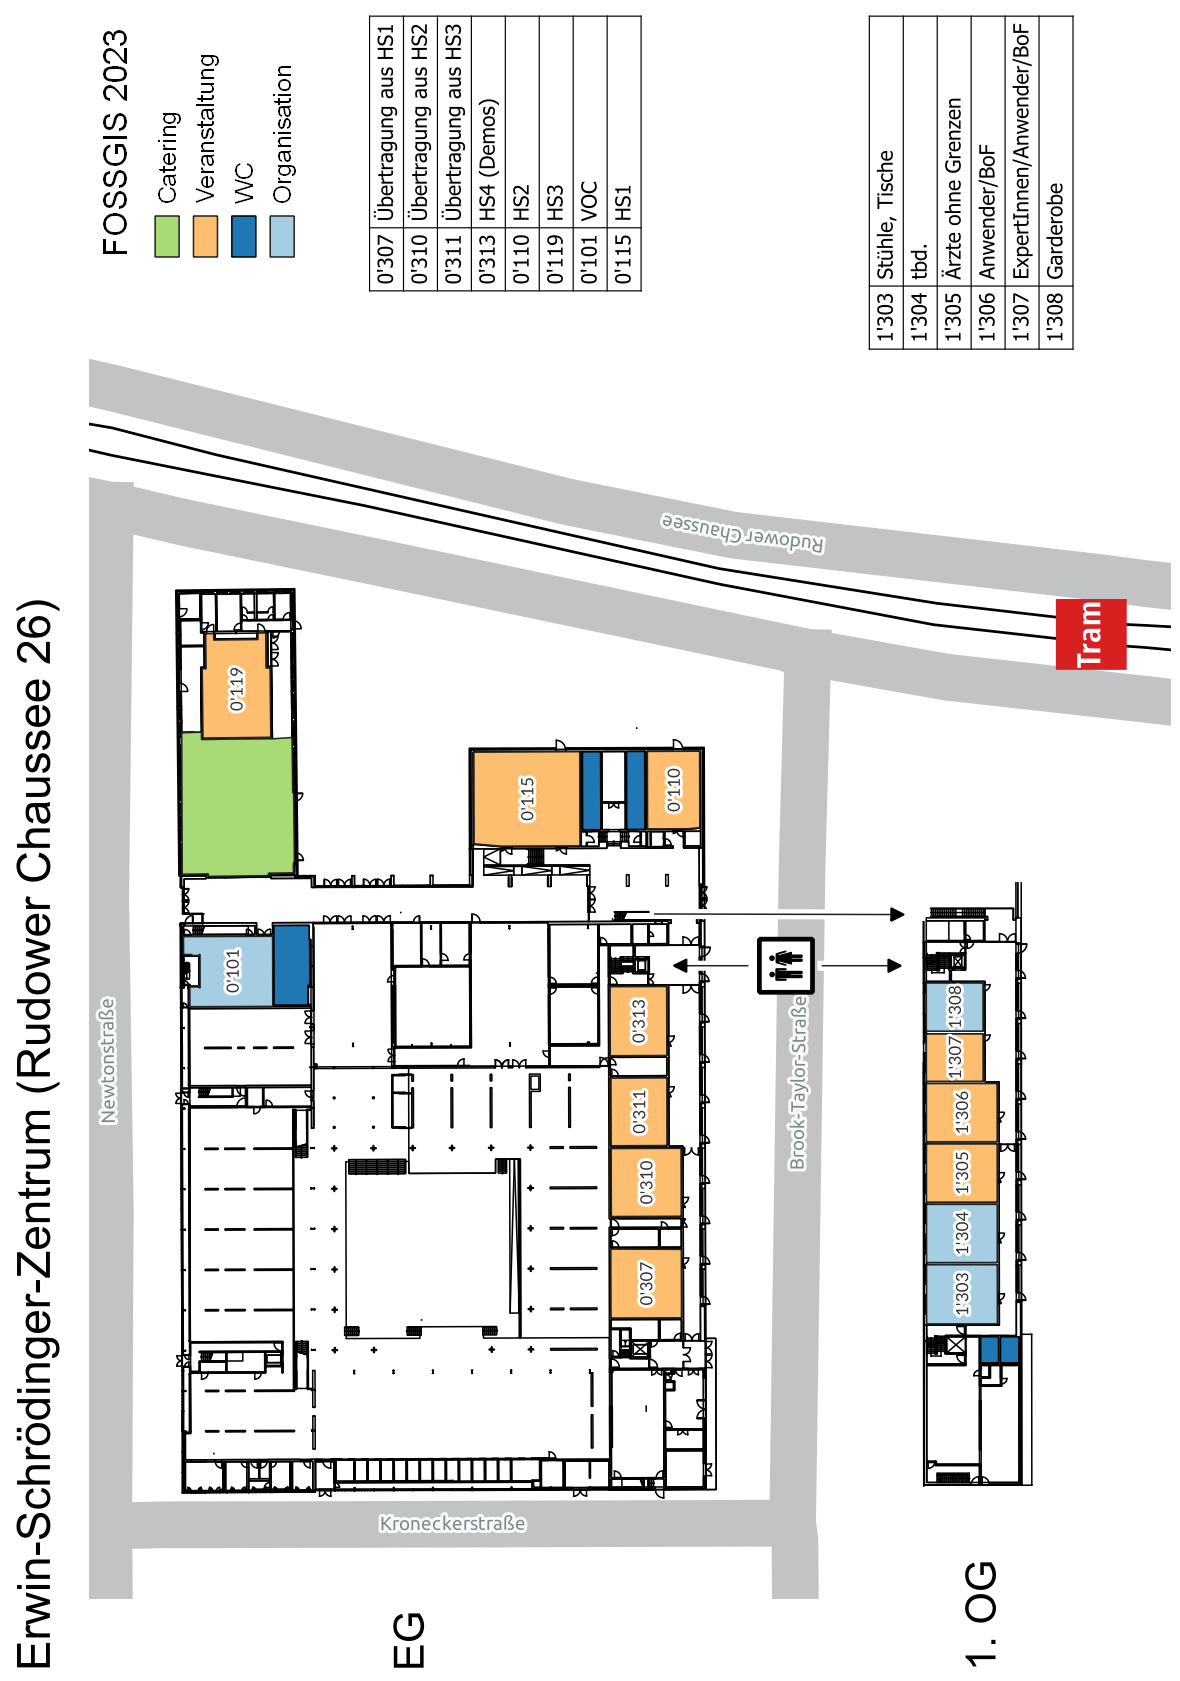
\includegraphics[height=158mm]{images-print/Raumplan_ESZ_RUD26.png}%
      };%
      \end{tikzpicture}%
   }%
]{esz}
\newpairofpagestyles[]{page-esz}{}
\AddLayersAtBeginOfPageStyle{page-esz}{esz}
\AddLayersAtBeginOfPageStyle{page-esz}{cropmarksplain}

% Raumplan Geographisches Institut
\DeclareNewLayer[background,%
  width=115mm,%
  height=158mm,%
  hoffset=5mm,%
  voffset=5mm,%
  contents={%
    \begin{tikzpicture}[x=1mm, y=1mm]%
      % map image
      \draw (0,0) node [inner sep=0mm, anchor=south west] {%
        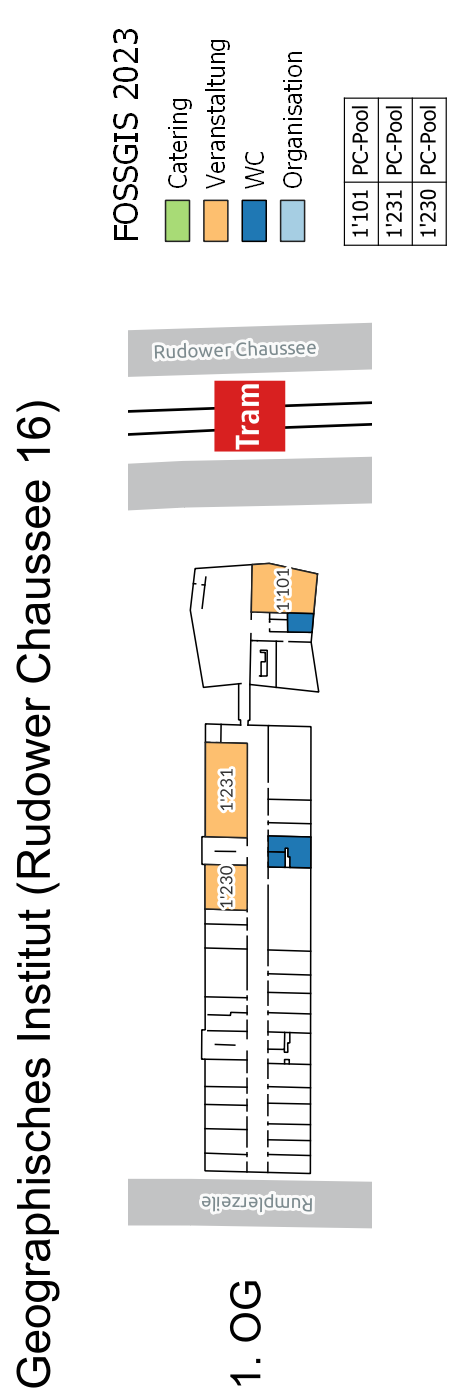
\includegraphics[height=158mm]{images-print/Raumplan_GI_RUD16.png}%
      };%
      \end{tikzpicture}%
   }%
]{gi}
\newpairofpagestyles[]{page-gi}{}
\AddLayersAtBeginOfPageStyle{page-gi}{gi}
\AddLayersAtBeginOfPageStyle{page-gi}{cropmarksplain}
